% $Id$
% ---------------------------------------------------------------------------
%
%  This is part of the SIGI.
%  Copyright (C) 2008 Interlegis
%  See the file relatorio.tex for copying conditions.
%

\section{Protótipo de Interface Gráfica}
\label{sec:prototipo}

\subsection{Tela de autenticação (login)}
O protótipo de interface para a autenticação no sistema pode ser
visualizado na Figura \ref{fig:login}.

\begin{figure}[h]
  \centering
  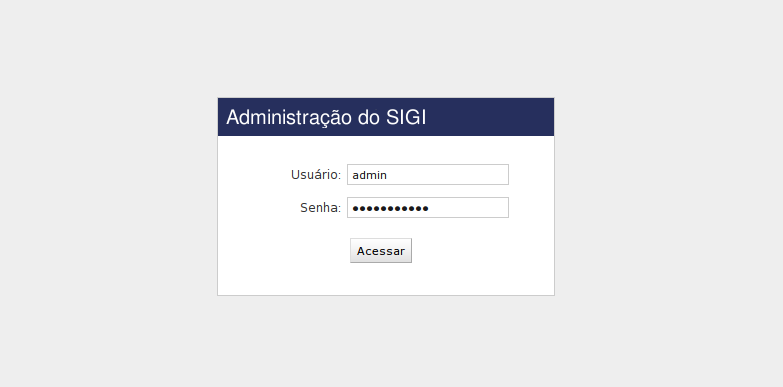
\includegraphics[width=100mm]{../imagens/telalogin.png}
  \caption{Tela para \textit{login} no sistema}
  \label{fig:login}
\end{figure}

\subsection{Dashboard}
Tela inicial do sistema após o \textit{login}, com informações gerais
e atividades recentes.

Um protótipo do \textit{dashboard} (painel) pode ser visualizado na
Figura \ref{fig:dashboard}.

\begin{figure}[h]
  \centering
  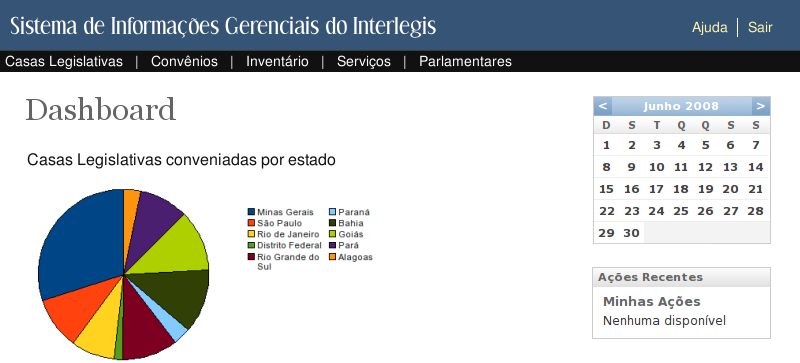
\includegraphics[width=120mm]{../imagens/dashboard.png}
  \caption{\textit{Dashboard}}
  \label{fig:dashboard}
\end{figure}

\subsection{Tela de cadastro}
O protótipo de interface para o cadastro de informações pode ser
visualizado na Figura \ref{fig:cadastro}.

\begin{figure}[h]
  \centering
  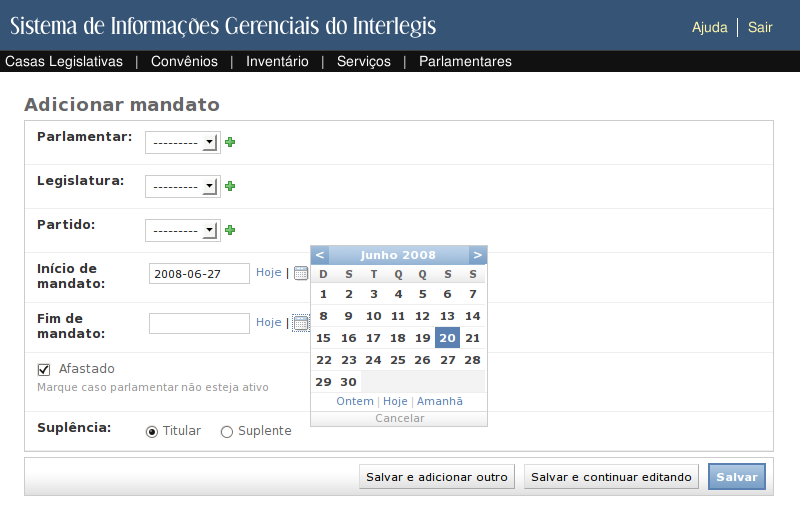
\includegraphics[width=120mm]{../imagens/cadastro.png}
  \caption{Tela de cadastro}
  \label{fig:cadastro}
\end{figure}

\subsection{Tela de listagem de dados}
O protótipo de interface para o listagem de dados pode ser visualizado
na Figura \ref{fig:listagem}.

\begin{figure}[h]
  \centering
  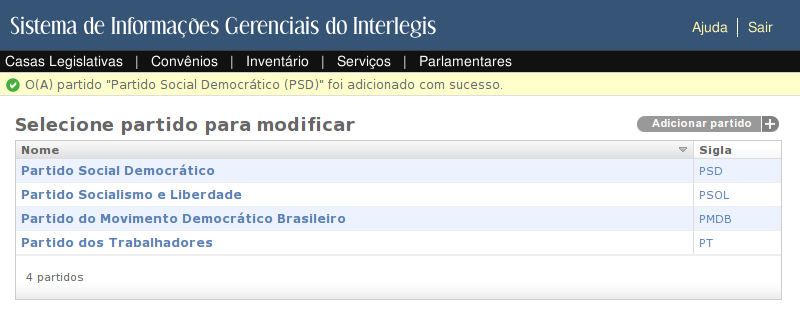
\includegraphics[width=120mm]{../imagens/listagem.png}
  \caption{Tela para a listagem de dados}
  \label{fig:listagem}
\end{figure}

%
% Local variables:
%   mode: flyspell
%   TeX-master: "relatorio.tex"
% End:
%
